\section{Projektplanl\ae{}gning}
Her gennemg\aa{}es essentielle projektplanl\ae{}gnings elementer. 

\subsection{Emnevalg}
I gruppen har der v\ae{}ret bred enighed om valg af emne. Retningen p\aa{} det emne var dog noget sv\ae{}rere at v\ae{}lge, men vi n\aa{}ede til en enighed hvor alle var tilfredse. 
Den endelige retning p\aa{} projekt blev f\o{}rst definitivt defineret meget sent i projektet.
Dette skyldtes at vi ikke fik lavet en grundig problemanalyse i starten af projektet.

Dette kan forbedres til P3 ved at lave en grundig problemanalyse i starten af projekt perioden. 

\begin{figure}[htbp]
\begin{center}
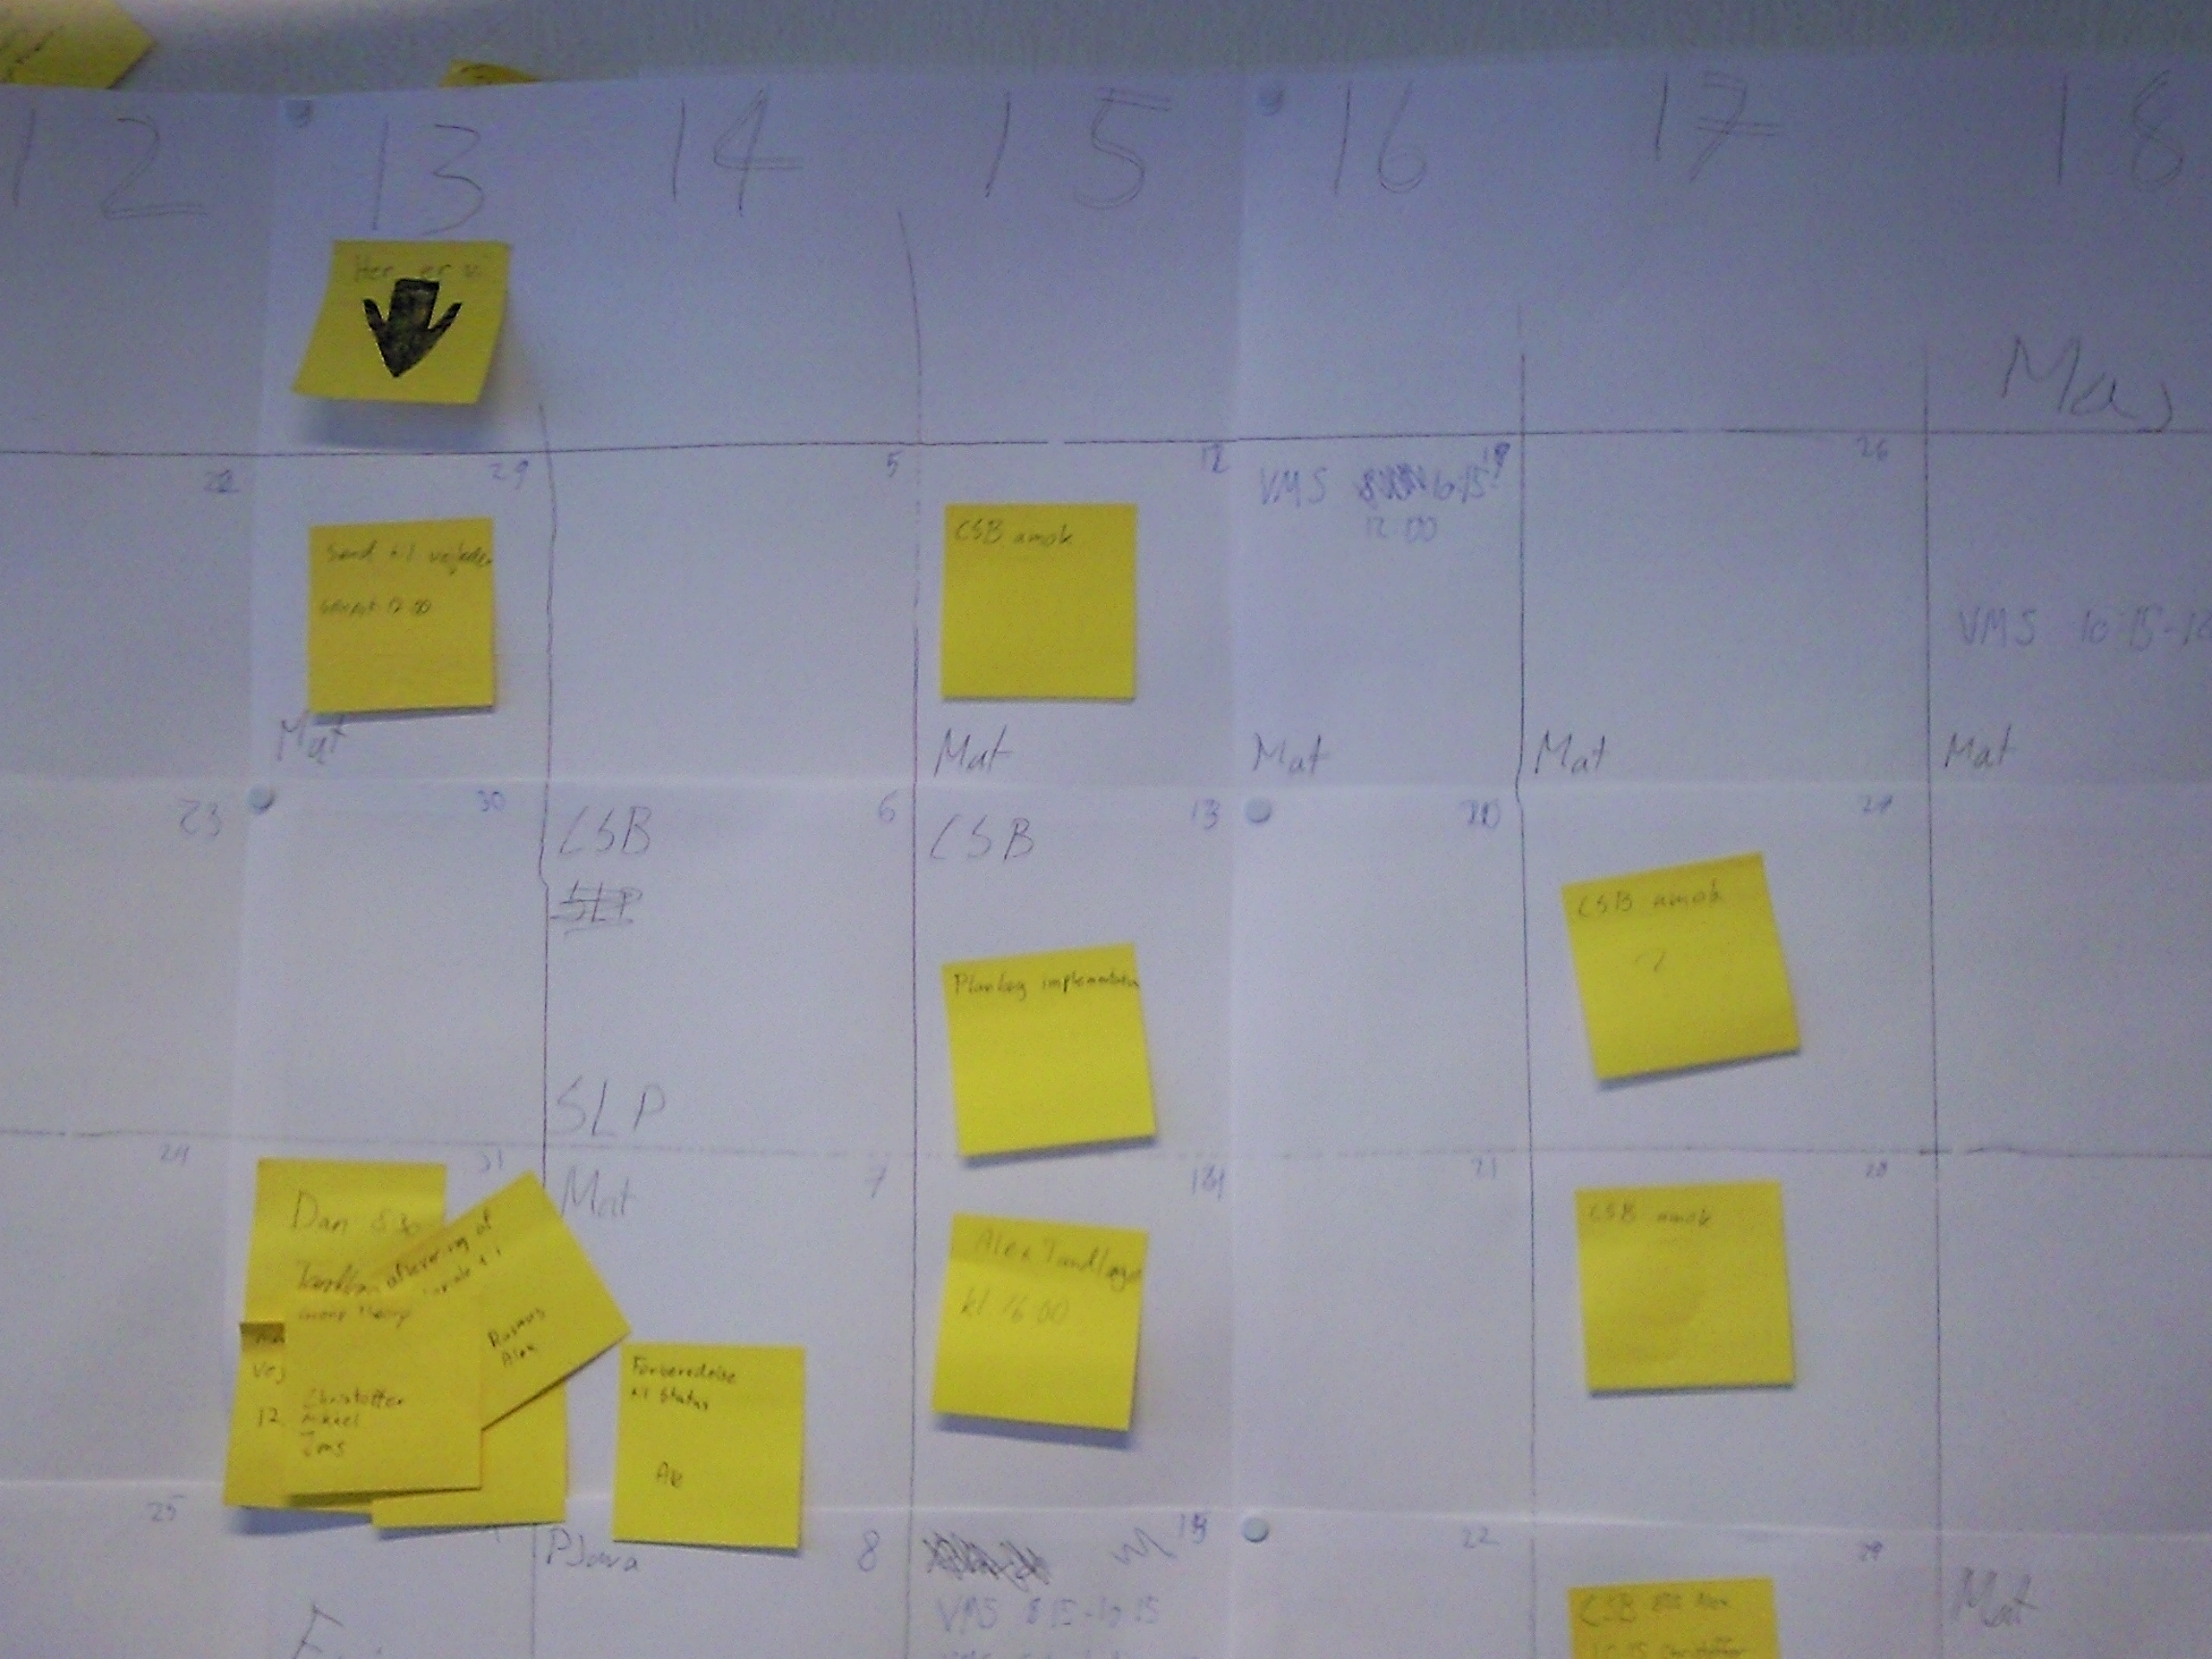
\includegraphics[width=\textwidth]{Billede0075.jpg}
\caption{default}
\label{default}
\end{center}
\end{figure}


\subsection{Tidstyring}
Til at administrere projektets arbejdsgang og tidsplan har vi anvendt en v\ae{}g kalender(see billede \ref{}), der fungerede b\aa{}de som opgavestyring og tidstyring. 

Kalenderen blev anvendt til at holde styr p\aa{} vores fastsatte deadlines. Hver opgave fik en post-it og blev opsat p\aa{} den dag hvor opgaven har deadline. Dette gav en stor fleksibilitet hvis opgavens omfang var fejlvurderet og den p\aa{}kr\ae{}vede tid til l\o{}sningen var st\o{}rre end f\o{}rst antaget, kunne post-it flyttes til en ny dato. 
 
I gennemretnings perioder virkede kalenderen dog ikke hensigtsm\ae{}sigt og vi anvendte tavler til styring af hvilke rapport elementer der blev retter af hvem. 
Kalenderen fungerede hensigtsm\ae{}ssigt og gav et l\o{}bende overblik over hvor i projektet vi stod og hvordan vi er med i forhold til deadlines. 

Til senere projekter kan et lignende system anvendes. Evt. en digitaliseret version da vores version optog meget v\ae{}g plads og en digitaliseret version kan tilg\aa{}s hjemmefra. 

\subsection{Projektstyring}
I gruppen valgte vi en flad demokratisk styringsform. Denne fungerede fint; alle emner og problemer blev diskuteret l\o{}bende. Dette var muligt da vi arbejdede stort set udelukkende i grupperummet og derved altid havde mulighed for at diskutere problemstillinger med hverandre. 

Vi har i projektet haft nogle roller, herunder; vejlederkontaktansvarlig, kontorkontaktansvarlig, trykkerikontaktansvarlig, kasserer, referent. Disse roller er delvist udefineret og nogle har v\ae{}ret skiftende roller.

Til P3 kunne der eksperimenteres med en defineret skiftende lederrolle for at opn\aa{} nogle lederkompetencer til alle gruppens medlemmer. 






